
% this file is called up by thesis.tex
% content in this file will be fed into the main document


\graphicspath{{6/figures/}}

\chapter{From Music Audio to Guitar Tablature}
\label{chp:background}

In the previous chapter, it was demonstrated that state of the art ACE systems are actually performing at a relatively high level, often producing reasonable chord estimations, if not the \emph{precise} labels of a reference annotation.
Deploying these systems in the wild for real users, however, presents two practical difficulties:
one, performing a given chord sequence requires that the musician already knows both the notes in each chord and how to play them on some instrument;
and two, classification-minded chord estimation systems do not degrade gracefully, e.g. produce ``next best'' answers.
Recognizing that many in the online music transcription community are guitarists, both challenges are addressed here by modeling the physical constraints of guitar's fretboard with a deep convolutional network to produce \emph{human-readable representations} of music audio, i.e. tablature.

Importantly, estimating the likelihood of hand positions on a fretboard entails a variety of advantages.
Guitar chord shapes impose an explicit hierarchy among notes in a chord family, such that related chords are forced to be near-neighbors in the output space.
This acts as a constraint on the learning problem, and encourages the model to learn musically meaningful outputs beyond the space of chords seen during training.
The human-readable nature of the system's output is also valuable from a practical perspective, being immediately useful with minimal prerequisite knowledge.
This further supports the goal of graceful degradation, such that a softer prediction surface results in more informative errors.
Finally, directly estimating playable represenations allows non-experts to easily validate system outputs and even correct errors.

% This paper presents a novel approach to bootstrapping the task of automatic chord recognition to develop an end-to-end system capable of representing polyphonic music audio as guitar tablature by modeling the mechanics of the guitar with a deep convolutional network.
% To enforce playability, a finite vocabulary of chord shape templates are defined and the network is trained by minimizing the distance between its output and the best template for an observation.
% Experimental results show that the model achieves the goal of faithfully mapping audio to a fretboard representation, while still performing respectably as a chord recognition system.
% The output of the network is human-readable, allowing the system to be used by anyone regardless of musical ability.
% Additionally, trained networks are not constrained to any particular vocabulary, and are able to represent previously unseen chord shapes.

\section{Context}
\label{sec:context}


\begin{figure}[t!]

  \centering
  \centerline{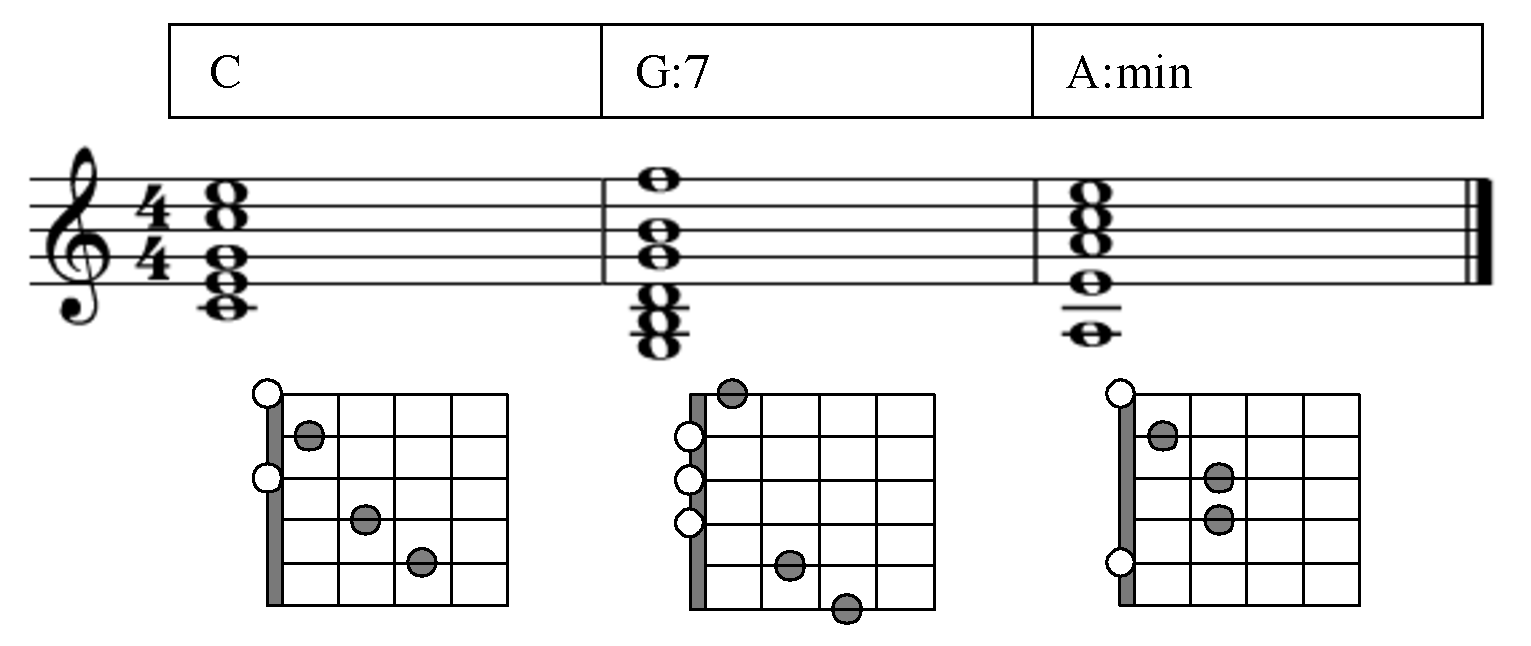
\includegraphics[width=\textwidth]{chord_tablature}}
\caption{A chord sequence (top), traditional staff notation (middle), and guitar tablature (bottom) of the same musical information, in decreasing levels of abstraction.}
\label{fig:chord_notation}
%
\end{figure}

% Rise of the guitarists
To date, the majority of research in automatic chord estimation is based on the two-fold premise that (a) this is fundamentally a classification problem, and (b) the ideal output is a time-aligned sequence of singular chord names.
That said, it is worthwhile to reconsider that the development of such systems is motivated by the goal of helping the amibitious musician learn to play any song\footnote{Any song that makes use of traditional Western tonal harmony, that is.}.
%TODO: This sentence blows. Fix it.
One of the largest groups of musicans attempting to do just that is the guitarist community.
Over the last century, the guitar, in all of its forms, has drastically risen in popularity and prevalance, both in professional and amateur settings.
Given the low start-up cost, portability, favorable learning curve, and undisputed ``cool factor'' in Western popular culture, courtesy of musicans like Jimi Hendrix or \emph{The Beatles}, it is unsurprising that guitars dwarf music instrument sales in the United States.
Based on the 2014 annual report of the National Association of Music Merchants (NAMM), a whopping 2.47M guitars were sold in 2013 in the United States, accounting for a retail value of \$1.07 \emph{billion} USD \cite{NAMM2014}; for comparison, \emph{all} wind instruments sales ---the next largest instrument category--- combined for just over half that figure, at \$521M USD.

% Tablature notation
While most instruments make use of traditional staff notation, fretted instruments, like lute or guitar, have a long history of using \emph{tablature} to notate music.
Illustrated in Figure \ref{fig:chord_notation}, tablature requires minimal musical knowledge to interpret, and thus offers the advantage that is easier to read, and generally preferred by beginners.
Whereas staff notation explicitly encodes pitch information, leaving the performer to translate notes to a given instrument, tablature explicitly encodes performance instructions for a given instrument and only implies pitch.
Though it can be difficult to accurately depict rhytmic information with tablature, this is seldom an obstacle for guitarists.
% It is typically easier to learn rhythm by ear than pitch.
Guitar parts often consist of chords strummed with little emphasis on rhythm patterns, and it is easy to align chord changes with lyrics or metrical position.
% Therefore, it is an inherent design challenge of human-facing expert systems that the output must be easily interpreted by the user; and, more importantly, graceful degradation is a function of that user's capacity to understand and recover from errors.

\begin{figure}[t!]
  \centering
  \centerline{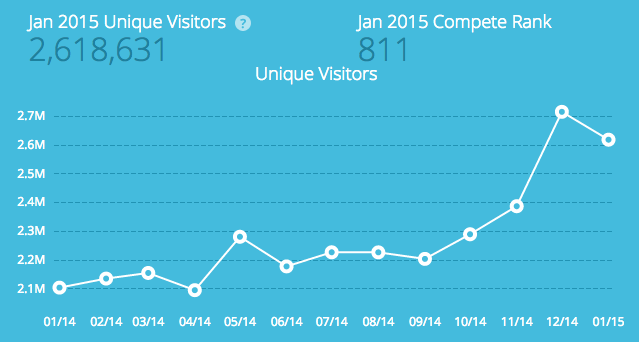
\includegraphics[width=0.8\textwidth]{ug_compete}}
\caption{Visitor statistics for the tab website \emph{Ultimate Guitar}, as of January 2015.}
\label{fig:ug_compete}
%
\end{figure}

% Digitization and the internet
As both personal computers and access to the Internet became more common, guitarists began to embrace technology for the purposes of learning to play popular music.
Bandwidth and memory limitations, however, prevented the curation of high resolution images of sheet music, and symbolic representations, like MIDI, required specialized programs to render the music visually.
With small filesizes and compatibility with common text editors, ASCII ``tabs'' made it comparatively trivial to create, share, and store guitar music.
Thus, combining easy readability and a sufficient level of musical detail with technological constraints of the time period, guitar tablature spiked in popularity towards the end of the $20^{th}$ century.
Today, evidenced by heavily trafficked, user-curated websites like Ultimate Guitar\footnote{http://www.ultimate-guitar.com/}, modern online guitar communities continue to place a high demand on tablature.
Shown in Figure \ref{fig:compete}, this one website sees, on average, well over 2M unique visitors\footnote{Based on Compete.com analytics data, accessed on 15 March, 2015.} on a monthly basis in the United States alone.

% Put it together
Taken together, these observations tell an interesting story.
Guitarists comprise a significant portion of the global music community, and are actively creating and using tablature as a means of learning music.
It seems rather obvious to conclude that an automatic chord estimation system would be extremely valuable to this demographic, but such a system should be sensitive to the common preference for tablature.
Therefore, this is an effort to steer automatic chord estimation toward a specific application, in order to address a real pain point for a real user base.


\section{Proposed System}

Much of this work proceeds directly from previous efforts in automatic chord estimation.
The input leverages the same CQT representation, and is omitted from the discussion here.

Though some previous work embraces this position in the realm of transcribing guitar recordings \cite{Barbancho2012} or arranging music for guitar \cite{Hori2013}, there is, to our knowledge, no existing work in estimating guitar tablature directly from polyphonic recordings.


\subsection{Designing a Guitar Chord Esimator}
\label{subsec:design}

So far, this study has shown deep trainable networks have proven to be a versatile, powerful, and practical approach to solving complex machine learning problems.
Thus it is a particular advantage of deep learning that various end-to-end systems can be quickly developed, provided one can express its fitness as a differentiable objective function.
This high level design strategy is exploited here by modifying the convolutional neural networks of the previous chapter to produce an output representation that behaves like the fretboard of a guitar.

For clarity, the modern guitar consists of six parallel strings, conventionally tuned to E2, A2, D2, G3, B3, and E4.
The polyphony of a guitar can be anywhere from zero to \emph{six}, the condition in which all strings are plucked, strummed, or otherwise activated.
A guitar is also fretted, such that the different pitches produced by a string are quantized in ascending order, as a result of shortening the length of the vibrating string.
A continuous pitch range may be achieved by various means, such as bending the strings, but such embellishments are rare to the point of unnecessary when addressing chords.
Thus, for the purposes here, it can be said that each string only takes a finite number of states: off (\texttt{X}), open, (\texttt{O}), or a number corresponding to the fret at which the string is held down.
As a simplification, all chords will be voiced in the first seven frets, and therefore each string can have nine mutually exclusive states.

Framed as such, the strings of a guitar can modeled as six correlated, but ultimately independent, probability mass functions.
The common approach toward achieving this behavior is by passing the output of an affine projection through a softmax function, as described in Chapter \ref{chp:method}, yielding a non-negative representation that sums to one.
Starting with the first three layers of the ``XL'' model defined previously, six independent softmax layers are used to model each string independently, and concatenated to form a 2-dimensional heatmap of the fretboard:

\begin{align*}
\label{eq:softmax_layer}
\small
Z_i = f_i(X_{l-1} \vert \theta_i) = \sigma (W_i \bullet X_{l-1} + b_i), i \in [0:6), \theta = [W_i, b_is]
\end{align*}

\noindent The activation of the $i^{th}$ string, $Z_i$, is computed by projecting the output of the penultimate layer in the network, $X_{l-1}$, against the weights, $W_i$, and added to a bias term, $b_i$.
This linear transformation is normalized by the softmax function, $\sigma$, and repeated for each of the six strings.
The overall model is diagrammed in Figure \ref{fig:guitarnet}.


\begin{figure}[t!]
  \centering
  \centerline{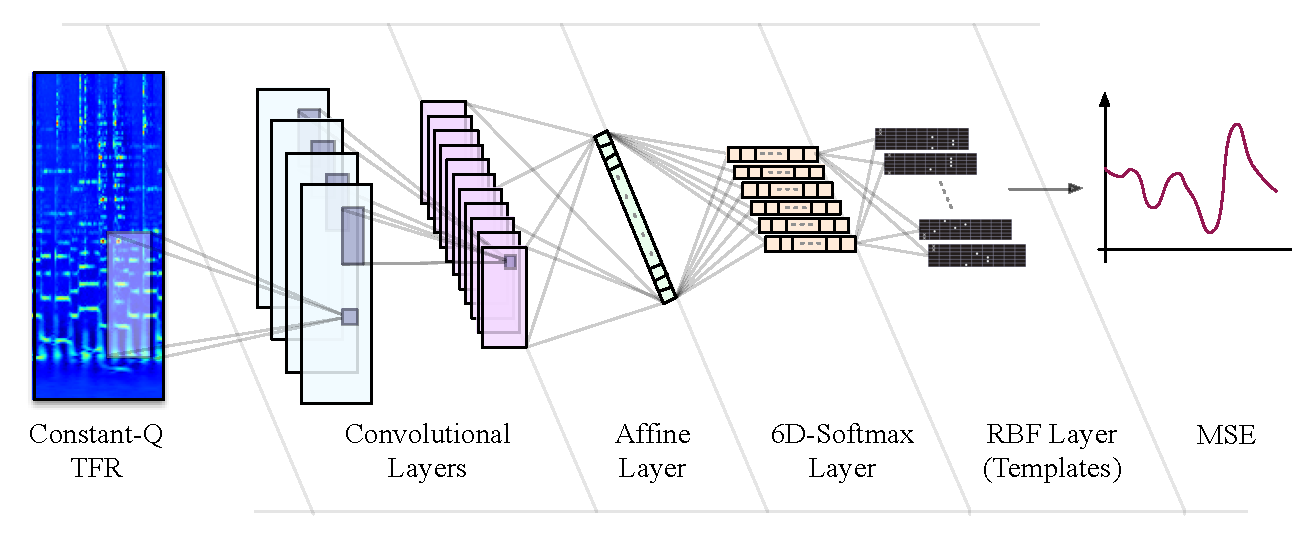
\includegraphics[width=\textwidth]{sys_diagram}}
\caption{Full diagram of the proposed network during training.}
\label{fig:guitarnet}
%
\end{figure}


\subsection{Guitar Chord Templates}
\label{subsec:vocabulary}

Having designed a convolutional network to estimate the active states of a fretboard, it is necessary to devise a mapping from chord transcriptions to fingerings on a guitar.
As the annotations available were curated for generic chord estimation, they  do not offer insight into how a given chord might best be voiced on a guitar.
Therefore, using the same vocabulary of 157 chords as before, a canonical chord shape ``template'' is chosen for each.
This is done in such a way so as to prefer voicings where all quality variations over a given root are maximally similar, i.e. chords of the same root are near-neighbors in fretboard space.
To illustrate, tablature representations for all templates are given in Figure \ref{fig:templates}.

It is worthwhile at this point to acknowledge the natural multiplicity of chord voicings on the guitar.
In addition to the normal variation that may occur in stacking the notes of a chord, e.g. ``open'' or ``closed'' position, there are other factors that influence the actual pitches that are played.
First, the same note can often be played in multiple positions on the fretboard.
For example, E3 can be played on the 12th fret of the first string, the 7th of the second, or the 2nd of the third.
Additionally, some standard chord voicings cannot be formed on the guitar, comfortably or otherwise.
As a result, it is common to play the 3rd degree of a chord over the octave, as the 10th, with a few exceptions resulting from open fingerings.
Perhaps most importantly, context is likely to determine how a chord is played, such that it is easier to move from one chord shape to the next.
Rather than attempt to cope with these issues now, the canonical template approach is chosen to simplify overall system design.
The choice of one template over another likely has nontrivial implications for the behavior of the model, but this is left as a variable to be explored in the future.


\subsection{Additional Prediction Functions}
\label{subsec:loss}

Before proceeding, there are two additional architectural considerations to be addressed.
First, the templates defined above must be incorporated into an objective function, such that the machine can learn to faithfully reproduce them.
Finding inspiration in \cite{LeCun1998}, a Radial Basis Function (RBF) layer is added to the network, given as follows:

\begin{equation}
\small
\mathcal{E}(Z \vert W_T) = \sum(Z_{out} - W_{T}[k])^2
\end{equation}

\noindent where $Z$ is the output of the fretboard model, $W_T$ is a tensor of chord shape templates with shape $(K, 6, 9)$, such that $K$ is the number of chord templates, and $k$ the index of the reference class.
Note that these templates will impose the proper organization on the output of the model, and thus remain fixed during the learning process.
Since these weights are constant, minimizing this function does not require a contrastive penalty or margin term to prevent it from collapsing, i.e. making all the squared distances zero.

Additionally, in order to apply Viterbi post-filtering and fairly compare with previous results, it is necessary to invert the energy surface into a likelihood function.
This is achieved by negating the energy function and normalizing as a Gibbs distribution:

\begin{equation}
\small
\mathcal{L}(Y_k \vert X, \Theta) = \frac{exp(-E(Y_k \vert X, \Theta))}{\sum_i^K~exp(-E(Y_k \vert X, \Theta))}
\end{equation}


\section{Methodology}

\subsection{Training Strategy}
\label{subsec:strategy}

It is critical to note that a fretboard prediction model cannot achieve root-invariant weight sharing as in the previous chapter, due to the nonuniformity of chord shapes with different roots.
To explore the impact of this shortcoming, three different training strategies are employed here.
As a baseline condition, the model is trained with the natural distribution of the data (``as-is'').
Note that this is expected to be a deficient condition, as there is chord class mismatch between training and test conditions, i.e. there are chord classes in the test partition that do not occur in the training set.
In the interest of addressing the imbalanced learning problem, the second training condition scales the loss of each training observation by a class-dependent weight (``scaled'').
These weights are determined by computing the root-invariant prior over the training partition, taking its inverse, and standardizing the coefficients to unit mean and standard deviation.
The third and final training condition couples loss scaling with data augmentation, such that during training each datapoint is circularly shifted in frequency on the interval $[-12, 12]$ (``augmented'').
This allows the variance of each chord quality to be evenly distributed across classes, and helping prevent any missing class coverage in the training set.

All models are trained with mini-batch stochastic gradient descent at a batch size of 50, learning rate of 0.02, and dropout ratio of 0.125.
Training proceeded for several hundred iterations, ultimately bounded by a ceiling of 24 hours.
Identical partitions of the dataset used in the previous chapter are employed here, and all results are averaged over five folds.


\subsection{Evaluation}
\label{subsec:evaluation}

In lieu of measuring subjective experience of using the system, the quality of the resulting models are evaluated at the same chord estimation task as in Chapter 5.4.


% \begin{table}[t]
% \begin{center}
% \scriptsize
% \caption{Micro-recall scores for }
% \label{tab:rc_agreement}
% \begin{tabular}{c|rrrrrrr}

% \hline
% \multicolumn{3}{l}{Cho, 2014} & & & & & \\
% \hline
%  & triads &   root &   mirex &   tetrads &   sevenths &   thirds &   majmin \\
% \hline
% Train & 0.8053 & 0.8529 &  0.8205 & 0.6763 & 0.6823 & 0.8261 & 0.8109 \\
% Test & 0.7970 & 0.8475 & 0.8147 & 0.6592 & 0.6704 & 0.8197 & 0.8057 \\
% \hline
% \hline
% \multicolumn{3}{l}{Unconstrained (Chapter 5)} & & & & & \\
% \hline
%  & triads &   root &   mirex &   tetrads &   sevenths &   thirds &   majmin \\
% \hline
% Train & 0.8899 & 0.9145 & 0.8962 & 0.8217 & 0.8214 & 0.9049 & 0.8908 \\
% Test  & 0.7995 & 0.8493 & 0.8145 & 0.6673 & 0.6788 & 0.8227 & 0.8077 \\
% \hline
% \hline
% \multicolumn{3}{l}{Fretboard Model} & & & & & \\
% \hline
%  & triads &   root &   mirex &   tetrads &   sevenths &   thirds &   majmin \\
% \hline
% Train & 0.8974 & 0.9240 & 0.9037 & 0.8136 & 0.8353 & 0.9098 & 0.9114 \\
% Test & \textbf{0.8234} & \textbf{0.8705} & \textbf{0.8352} & \textbf{0.6855} & \textbf{0.7084} & \textbf{0.8376} & \textbf{0.8394} \\
% \hline
% \end{tabular}
% \end{center}
% \end{table}

\begin{table}[t]
\begin{center}
\scriptsize
\caption{Micro-recall scores for two previous models, and the three training conditions considered here.}
\label{tab:rc_agreement}
\begin{tabular}{c|rrrrrrr}

\hline
 & triads &   root &   mirex &   tetrads &   sevenths &   thirds &   majmin \\
\hline
Cho, 2014 & 0.7970 & 0.8475 & 0.8147 & 0.6592 & 0.6704 & 0.8197 & 0.8057 \\
\hline
Unconstrained (Chapter 5)  & 0.7995 & 0.8493 & 0.8145 & 0.6673 & 0.6788 & 0.8227 & 0.8077 \\
\hline
As-Is     & 0.8234 & 0.8705 & 0.8352 & 0.6855 & 0.7084 & 0.8376 & 0.8394 \\
Scaled    & 0.8156 & 0.8644 & 0.8283 & 0.6791 & 0.6994 & 0.8308 & 0.8295 \\
Augmented & \textbf{0.8294} & \textbf{0.8715} & \textbf{0.8420} & \textbf{0.6989} & \textbf{0.7167} & \textbf{0.8440} & \textbf{0.8412} \\
\hline
\end{tabular}
\end{center}
\end{table}


\begin{table}[t]
\begin{center}
\scriptsize
\caption{Quality-wise recall across conditions.}
\label{tab:qualitywise}
\begin{tabular}{c|c|ccc|c}

 quality   &  Unconstrained &  As-is & Scaled & Augmented & Support (min) \\
\hline
 maj       &  0.7390 &  0.8572 &  0.8413 &  0.8417 &  397.4887 \\
 min       &  0.6105 &  0.6516 &  0.6312 &  0.6645 &  105.7641 \\
 7         &  0.5183 &  0.2928 &  0.3001 &  0.3367 &   68.1321 \\
 min7      &  0.5263 &  0.4556 &  0.4670 &  0.5077 &   63.9526 \\
 N         &  0.7679 &  0.6670 &  0.6712 &  0.6942 &   41.6994 \\
 maj7      &  0.6780 &  0.4143 &  0.4614 &  0.5525 &   23.3095 \\
 \hline
 maj6      &  0.2908 &  0.0259 &  0.0682 &  0.1061 &    7.6729 \\
 sus4      &  0.3369 &  0.0252 &  0.0952 &  0.1747 &    8.3140 \\
 sus2      &  0.3216 &  0.0098 &  0.0146 &  0.2216 &    2.4250 \\
 aug       &  0.5078 &  0.0093 &  0.1431 &  0.3365 &    1.2705 \\
 dim       &  0.4105 &  0.2898 &  0.4030 &  0.3803 &    1.8756 \\
 min6      &  0.3870 &  0.0367 &  0.1611 &  0.3011 &    1.5716 \\
 hdim7     &  0.5688 &  0.0000 &  0.0610 &  0.3913 &    1.1506 \\
 dim7      &  0.1790 &  0.0040 &  0.0453 &  0.0391 &    0.5650 \\
 \hline
 average   &  0.4887 &  0.2671 &  0.3117 &  0.3963 &  \\
\hline
\end{tabular}
\end{center}
\end{table}




\begin{figure}[t!]
  \centering
  \centerline{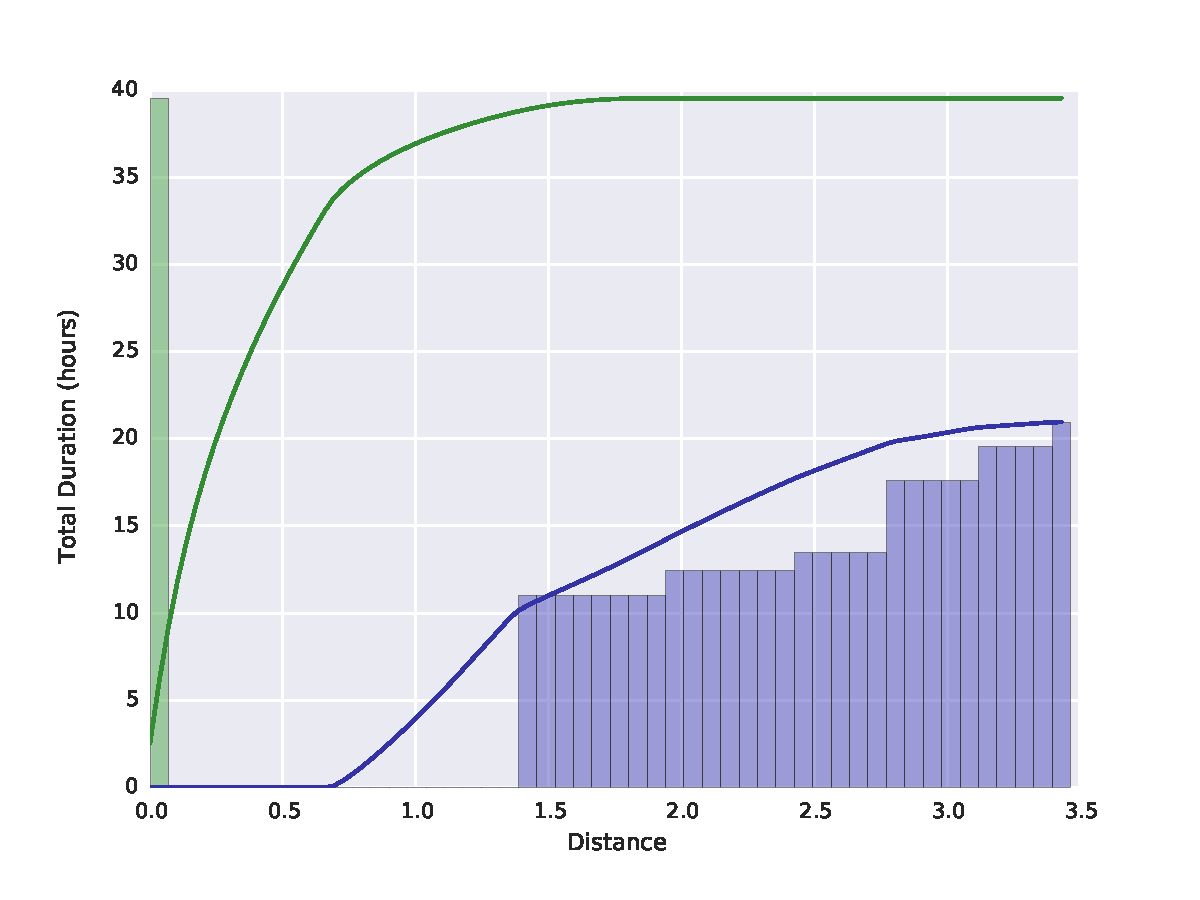
\includegraphics[width=\textwidth]{quant_error}}
\caption{Understanding classification as quantization error. Cumulative distribution functions are show for correct (green) and incorrect (blue) classification, in the discrete (classification) and continuous (regression) conditions.}
\label{fig:quant_error}
%
\end{figure}
